% ---------------------------------------------------------
\chapter{On Finding Performance Hot-Spots}
\label{chap:method}
% ---------------------------------------------------------

In the following, we provide an overview of our approach for finding performance hot spots. First, we frame our work on performance analysis in the context of configurable software systems. Then, we present existing performance-monitoring techniques we used in this thesis. We compare different monitoring tools regarding their accuracy, monitoring overhead, and other properties. Based on this analysis, we select the \ac{JIP}, which we use for implementing our approach. Afterwards, we describe how to sample configurable software systems to obtain a set of measurements that we use for learning a performance-influence model.

\section{Problem Statement}

% What is the problem now with performance analysis on method level and configurable software systems?
% What can be done?

% Let experts or developers configure the system. Drawback - reconfiguration of software systems each time, the software changes. May be also infeasable.

Today, almost every software system is configurable. Such software systems offer a huge amount of configuration possibilities. To facilitate the usage of such systems, they were provided with default configurations making it easier for users to utilize them. It is common practice that default configurations are designed by experts or developers themselves. Due to the evolution of source code which comes with adoption of requirements and the development of new features, the configuration space might grow and provided default configurations need to be adapted. Even domain experts are overwhelmed to get through the huge amount of possibilities and constraints which arise thereby.

Existing performance analysis tools (like the ones we presented in section~\ref{rel_perf_java}) lack the possibility to incorporate configurability into their analysis. They are often applied only to default configurations. Because it is not feasible to analyze each variant of software with such tools, many configuration possibilities remain untested. This leads users to stick to default configurations, because of the sheer size of possibilities to configure them. Furthermore, if they configure their systems, they might face performance problems which are still undiscovered, due to the lack of performance tests which aim at analyzing performance bugs of configurable software systems. The state of practice of performance testing in Java-based \ac{OSS} projects was conducted by~\cite{leitner2017exploratory}. They analyzed 111 projects from GitHub, trying to identify to which extend these software projects take care of their performance. They found that in 48\% of the projects only a single developer is responsible for creating and maintaining performance tests. They also discovered that 14\% of the analyzed projects have only a single commit for performance tests. The median number of commits for performance tests is 7, which indicates that many \ac{OSS} projects do not actively maintain performance tests. If this study can be generalized to other \ac{OSS} projects, the lack of analyzing and dealing with performance problems is an important problem, which has to be solved.

However, we are able to learn the influence of configuration options on performance by using variability modelling (existing approaches are presented in Section~\ref{rel_perf_pred}). But until now, they are just able to learn performance of variants of software systems as a whole (black-box approach). Existing variability modelling techniques (see section~\ref{background_variab_models}) lack the possibility to pin point performance hot spots or performance bugs to parts of software or to a specific code position.

% systeme, die das verbinden
% aber ... es wird benötigt

% \cite{Han:2016:ESP:2961111.2962602}
% configuration space includes interaction with other system components: shared libraries, environment variables, and kernel modules
% cause of performance bugs: complexity of configuration space and sophisticated constraints among configuration settings
% Comparison to functional bugs: typically leads to system crashes or incorrect results
% performance bugs can lead to significant performance degration, poor user experience, long response time, and slow system throughput
% they are more difficult to handle because they manifest themself often only with large inputs and in specific anvironments

% The main question developers should ask is: to what extend performance bugs remain undetected if only default configurations are tested
% Maybe some configuration options are more likely to trigger performance bugs than others
% they found out that more then half of the performance bugs are caused by configuration problems
% best case for performance testing analysis: the workload (load tests) is defined/provided/described by the developers themself. 

% performance bugs are most to be solved by code changes


Currently, there are neither white-box tools for performance-bug detection nor white-box tools for performance analysis of highly configurable software systems. However, there is an increasing need of such support. 
\cite{Han:2016:ESP:2961111.2962602} conducted an empirical study on performance bugs of configurable software systems. They wanted to investigate to what extend performance bugs remain undetected if only default instances are tested. If there are only a few performance bugs caused by configurations, developers might stick to classical performance analysis of default instances. But if there is a relevant portion of performance bugs sensitive to configuration options, it might be worth exploring these configurations further. Therefore, they investigate 113 real-world performance bugs randomly sampled from \ac{OSS} projects (e.g. Apache\footnote{Apache is one of the most used HTTP server~(\cite{apache2018url}).}, MySQL\footnote{MySQL is the world's most popular \ac{OSS} database~(\cite{mysql2018url}).}, Firefox\footnote{Firefox is a leading web browser~(\cite{firefox2018url}).}). They found that 59\% of performance bugs are related to configuration settings, whereas 41\% of the bugs are general performance bugs. Another observation was that all studied performance bugs result from legal configuration options (options that are in the valid part of the configuration space). Moreover, they analyzed how these performance bugs were fixed. There are two possibilities how fixing can be done: first, through changing configuration values, and second, through patching the source code. A majority of the 113 bugs of their study were patched through adapting the source code of the projects. On top of that, fixing general performance bugs needs to adapt 8 lines of code, on average, whereas patching performance bugs related to configuration options needs adaptation of 30 lines of code, on average. That means fixing configuration-related performance bugs is associated with more effort. Providing tools which are able to support performance bug analysis is all the more important, the more complex software systems become.


\section{Overall Process}
\label{overall_process}

\begin{figure}
  \centering
  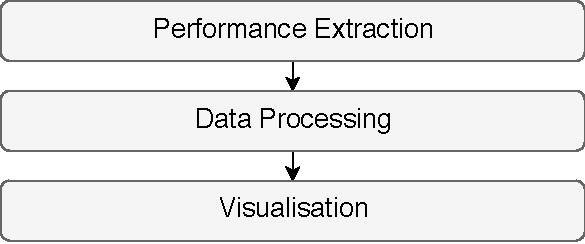
\includegraphics[width=0.7\textwidth]{images/workflow_overview_0}
  \caption{Performance Analysis Workflow.}
  \label{big_picture_perf_anal_workflow}
\end{figure}

% Overview of the process
We divided our approach into three parts as shown in Figure~\ref{big_picture_perf_anal_workflow}. First, we extract the performance data from our subject systems (see Section~\ref{perf_extr})by executing each system in different configurations using different workloads in our test environment, which we describe in section~\ref{test_env}. To obtain a list of configurations, we use different sampling techniques as described in Section~\ref{perf_measure_sampling}). During execution, we profile the execution of the Java program of the corresponding configuration and obtain a fine-granular output describing the execution times of each method. For profiling, we compared different monitoring tools, as described in Section~\ref{monitoring_tools}, and decided for the tool \ac{JIP}. In the second step we process the collected data. An important part is the training of a regression model per method that allows us to predict a method's execution time for unseen configurations. The last step of our approach focuses on analyzing the performance hot spots via visualizations of the collected performance data (described in section~\ref{visualisation}). To this end, we designed an Eclipse plugin to visualize performance hot spots through the \ac{IDE} directly in the source code. Additionally, we developed a graph-based visualisation to give an overview of the influence of configuration options and their interactions on the performance of the subject systems.


\subsection{Performance extraction}
\label{perf_extr}

\begin{figure}
  \centering
  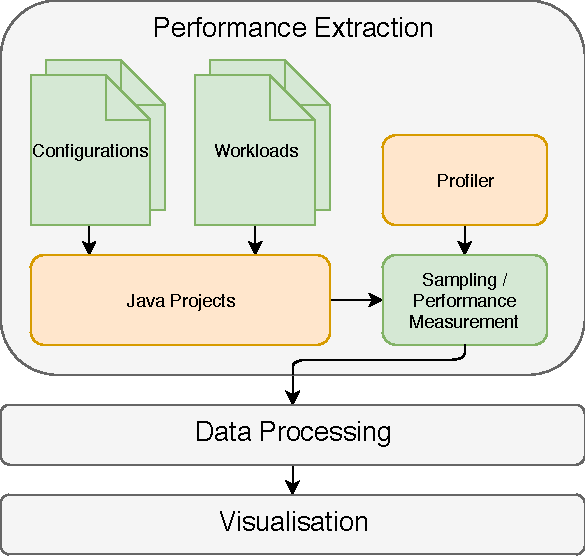
\includegraphics[width=0.7\textwidth]{images/workflow_perf_expanded}
  \caption{Performance Extraction Worklow.}
  \label{perf_extr_workflow}
\end{figure}


Next, we explain how we extract the performance data from configurable software systems; Figure~\ref{perf_extr_workflow} provides an overview. The orange parts of this diagram represent existing tools we used for this thesis and the green parts are results of our implementation. For the evaluation, we have chosen three Java projects from GitHub as case studies, which we describe in Section~\ref{case_studies} in more detail. The main tasks that we have addressed here are: selecting which configurations to measure, seelecting a suitable benchmark as a representative workload for executing a variant (i.e., the program that corresponds to a specific configuration), and preparing the environment for reliable measurement. In order to measure performance during execution, we used the \ac{JIP}. This profiler is able to measure the runtime of each method during execution of the software. However, we have to deal with the influence of non-determinism that affect overall performance. Our measurements run on real hardware in a \ac{JRE} with other processes being executed in parallel. 

%Because software runs on real hardware, the measurements might be influenced by a measurement bias. Hence, we want to find out if and to which degree the environment has an influence on performance. We also trained a regression model that aims on predicting the performance of each method depending on given configurations. An introduction to linear regression and an overview of the tools we used for modelling can be found in section~\ref{lin_reg}. 

\subsubsection{Sampling}
\label{perf_measure_sampling}

Sampling is the selection of a subset of individuals to estimate characteristics of the whole population. In the context of configurable software systems, the goal is to select individual configurations from the whole configuration space in order to reduce the amount of samples we have to analyze while not degrading the accuracy of the analysis. There are various sampling strategies, which all have different application areas and purposes. One criterion, which influences the choice of a sampling strategy, is the number of dimension that define the configuration space. 

With an increasing number of dimensions, also the volume of the space increases and the sampled data becomes sparse. This sparsity is problematic for any method that requires statistical significance. In order to obtain a statistically sound and reliable result, the additional amount of data needed to support the result often grows exponentially with the dimensionality. This phenomena is called \textit{Course of Dimensionality}~(\cite{donoho2000high}).

Furthermore, each individual dimension could represent a different type of data~(\cite{stevens1946theory}). There are four measurement scales: nominal, ordinal, interval, and ratio. Nominal data are used for labeling data. Usually nominal data is mutually exclusive and none of them have any numerical significance. A special type of nominal scale is binary data (e.g., on/off, true/false). With ordinal data, we can order the values, but the difference between them is not known (e.g., good, OK, bad). Whereas with interval scales, the ordering as well as the exact difference between the values is known (e.g., temperature scale). Moreover, ratio scales define the ordering, the distance, and also the absolute zero of the values (e.g., height or weight). In the context of configurable software systems, we have to be able to sample each of these dimensions to get a configuration. This is one reason why different sampling strategies were developed. Usually there are two types of data which are used for configuration: binary and numerical values. There are strategies for each of this two types of data, as presented in section~\ref{rel_perf_pred}.

We choose \textit{Random Sampling} as our sampling strategy, because with it we do not need to know the type of data which we want to sample. Random sampling is only possible because our subject systems does not have any constraints among configuration options. With random sampling we pick one value equally distributed from the values we could choose from. So for each dimension we have to know the start and end value and the step size in between. One drawback of this approach is that the range of each dimension has the same size, even two values in one dimension and thousands of values in another. 
\todo{Maybe extend database example and print:}
\todo{Example Sampling of 10 bin and 5 numeric}
\todo{Construction of Configurations}


%Random Sampling

%\todo{Maybe Binary Sampling Strategies}
%\subsubsection{Binary Sampling}
%Option-Wise  t  c  e s p  a   
%Negative-Option-Wise
%t-Wise
%Binary-Random
% Why random ... other paper.

%\todo{Maybe Numeric Sampling Strategies}

%\subsubsection{Numeric Sampling}
%One Factor at a Time
%Central Composite
%Placket-Burman Design
% other strats
% Distance computation



\subsubsection{Java Monitoring Tools}
\label{monitoring_tools}

Measuring performance of software is an important aspect of \ac{SPE}. Many monitoring tools were developed which extract performance values such as hit rate, memory consumption, and runtime. For this thesis, we examined a variety of monitoring tools for Java programs. In order to justify the decision to use \ac{JIP} for measurements, we compare existing tools.

\begin{sidewaystable}
% Include Profiling Overhead and Accuracy to table

	%\centering % Center table
    \begin{tabular}{*{9}{c}}
    	\toprule
        Tool & Performance Type & Resolution & Realization & Version & Filter & Output & Overhead \\
        \midrule
        NetBeans Prof. & \makecell{runtime, heap, \\ SQL queries, \\ threads} & \makecell{Windows 10 ms \\ Linux 10 ms \\ Solaris 1 ms} & aspect & J2SE 5.0 & yes & NetBeans GUI & --- \\
        \midrule
        VisualVM & \makecell{runtime, heap, \\ threads, GC} & snapshot & aspect & J2SE 5.0 & yes & VisualVM GUI & --- \\
        \midrule
        HPROF & runtime, heap & 1 ms & JVMTI & J2SE 5.0+ & yes & txt & 0.0\% \\
        \midrule
        Patty & \makecell{runtime, heap, \\ threads, GC} & 1 ms & JVMTI & J2SE 5.0 & yes & GUI, txt & --- \\
        \midrule
        JIP & runtime & 1 ms & aspect & J2SE 5.0+ & yes & txt & 0.0\% \\
        \midrule
        Profiler4J & \makecell{runtime, heap, \\ threads} & --- & JVMTI & J2SE 5.0 & yes & GUI & --- \\
        \midrule
        JRat & runtime & 1 ms & JVMTI & J2SE 5.0 & yes & GUI & --- \\
        \midrule
        EJP & runtime & --- & JVMPI & J2SE 1.4.2 & no & GUI & --- \\
        \midrule
        JMeasurement & runtime & 1 ms & source code & J2SE 5.0 & yes & txt, csv & --- \\
        \midrule
        DJProf & runtime, heap & 5 ms & aspect & J2SE 5.0 & no & txt & --- \\
        \midrule
        Kieker & runtime, heap & 1 ms & aspect & Java SE 7 & no & txt & 0.0\% \\
        \midrule
        SPASSmeter & runtime, heap & 1 ms & aspect & Java SE 7 & no & txt & 0.0\% \\

        %JRMC & B & C & D & B & C & D \\
        %\midrule
        %JMP & B & C & D & B & C & D \\
        %\midrule

        \bottomrule
    \end{tabular}
    \captionof{table}{Survey of Java Monitoring Tools.}
    \label{java_monitoring_tools}
\end{sidewaystable}

Table \ref{java_monitoring_tools} provides an overview of selected Java monitoring tools. We examined only \ac{OSS} tools, because these tools are free to use for all. We also searched explicitly for tool which work on terminal level when executing a Java program, because we want to automate the process of performance extraction. The following describes the six properties we used for comparison:
\begin{description}[style=multiline,leftmargin=8em]
	\item [Tool] is the name of the monitoring tool.
	\item [Performance Type] summarizes the performance data types that could be extracted with the tool.
	\item [Resolution] identifies the possible sampling rate of the tool.
	\item [Realization] states with which technical implementation the data extraction is realized.
	\item [Version] shows the Java version which is documented with the tool.
	\item [Filter] indicates whether with this tool there is the possibility for defining packages or classes from which the data should or should not be collected.
	\item [Output] what kind of data can we get from the tool. 
\end{description}


We searched for performance monitoring tools, that are able to extract the runtime of a method. In total, we have found twelve tools as shown in Table~\ref{java_monitoring_tools}. Some tools are able to extract also other types of performance data, but for this thesis, we are interested only in runtime. 

\textit{Resolution} (sampling rate) is the first property on which the tools differ. Most of the tools have a resolution of 1 ms. Exceptions are VisualVM which samples only snapshots initiated by the user, DJProf, which has a resolution of 5 ms, and NetBeans Profiler, which is ten times slower than the others on Windows and Linux. Both monitoring tools are too inaccurate for our purposes. 

The realization of the measurement is important in our context, because we want to automate the process of performance extraction. Four tools use \ac{AOP} to insert functionality for profiling. Five tools use an interface provided by to \ac{JVM}. The JVMPI interface is since J2SE version 1.5 the predecessor of the JVMTI interface. Both are used to inspect the state and to control the execution of applications running in the \ac{JVM}. But JVMPI was always labeled as a native experimental profiling interface and is deprecated since JVMTI was released, hence, EJP does not work any more with todays Java versions.

The column \textit{Version} repeats the version which is written in the documentation of these tools. This information aligns the tools with the development progress of the Java language.

A possible effect on the monitory accuracy represents our extensions that we made to the subject systems in order to input different configurations. Ideally, we want to exclude this extension from profiling to measure only the performance of the software itself. So, the tool we use has to have the possibility to filter specific classes, hence EJP and DJProf are excluded.

Four out of ten tool present their data only in a \ac{GUI}. Graphical representations might be helpful if there are information needed at once. But, we want to analyze a large number of configurations, so we have to automate the analysis process. Therefore, we want to have the results in a textual representation (e.g., txt, csv), which excludes NetBeans Profiler, VisualVM, JRat, Profiler4J, and EJP. 

%Profiling overhead.
%Accuracy of extracted data.
\todo{results}
Finally, we analyzed the Java monitoring tools. That is, we measure the overhead of HPROF, Kieker, SPASS-meter and JIP. To this end, an experiment, in which we randomly selected 100 configurations from each subject system and repeated measurements five times with and without monitoring. Based on this comparison, we calculated the introduced relative overhead and show it in the last column of Table x.
We can see that the tools X, Y, and Z introduce a substantial overhead such that these tools cannot give us reliable performance values. Only tools X,Y have low overhead so that we decided for tool X as it has all features that we need for our scenario.


\subsection{Data Processing}
\label{data_prozessing}

Next, we describe how we process the obtained data, as summarized in Figure~\ref{data_processing_workflow}. After monitoring each of the subject system, we have several Performance log fines containing execution times for each method. We obtain one log file for each subject system, each configuration, and each applied workload (a simplified log file can be found in appendix~\ref{example_log_file}). Each log file is divided into three sections with different information. The head of the file shows the time stamp of the file as well as the path to the file itself. We decoded the used configuration and workload in the path. The second area shows an inter-procedural control-flow graph\footnote{Inter-procedural control-flow graphs are tree structured graphs representing the control flow of a program.} which represents calling relationships between the individual methods of the subject systems. Each line is made up of the number of calls, the time spent in the method, and the method name with the fully qualified class name. The last section contains a list of all methods which are sorted by their net time\footnote{Net time is the amount of time that was actually spent executing this method. Here, the time taken by calling other methods is factored out.}. Based on these log files, the data processing is divided into three steps: analyzing the measurement influence, calculating relative performance of methods, and creating performance-influence models.


\begin{figure}
  \centering
  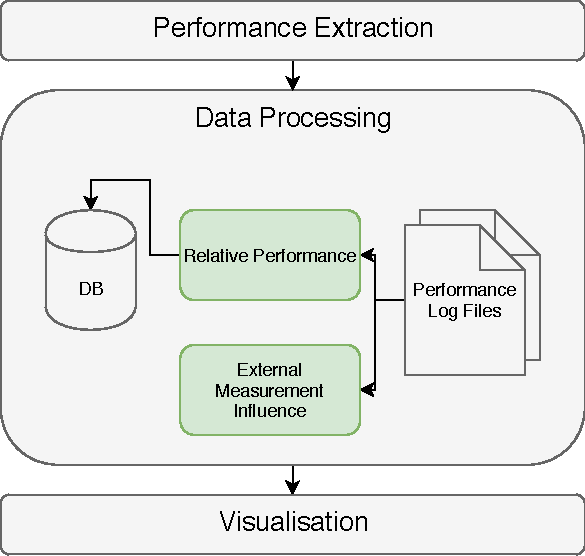
\includegraphics[width=0.7\textwidth]{images/workflow_data_expanded}
  \caption{Data-processing Worklow.}
  \label{data_processing_workflow}
\end{figure}


\subsubsection{External Measurement Influences}

Extracting actual performance values from configurable software systems requires executing the system under a specific configuration, workload, and environment. The execution environment is defined by th used hardware setup, an \ac{OS}, installed software, and several system settings. To enable reproducibility, we will delimit the measurement setup in Section~\ref{test_env}. Every part of the environment might have an influence on our measurements. This might be a source of non-determinism, which influences the whole process of performance analysis. Therefore, we try to minimize this influence in an two-step approach: Reduce system influence and .

\paragraph{System Influences.}
\label{perf_measure_system}

First, we try to reduce the influence of the system on our measurement. Therefore, we use separate machines dedicated to measure all test cases of an individual subject systems. Further, we ensured that there is only software installed which we need for the measurements. We restrict the execution of the measurement to one dedicated CPU core, because the hyper-threading feature of modern CPUs tries to balance the work between all available CPU cores, with the drawback that assigning a process to a specific core consumes additional, non-deterministic time. Another property of current CPUs is their ability to overclock. This allows the CPU to temporarily increase their clock frequency for different parts of the software execution. Again, this overclocking features results in non-deterministic performance behaviour and so we turned it off in our experiments.

%Sources of non-determinism whole measuring performance.
%Environment in which software is executed is defined by hardware, \ac{OS}, software and system settings.
%Processes and threading is also a matter if on multi core machine.

\paragraph{Java Measurement Influences.}
\label{perf_measure_java}

%paper: \ref{georges2007statistically}

Profiling of software that is executed in a runtime environment, such as the \ac{JVM}, is affected by additional factors that influence performance. With Java, the source code first need to be compiled into platform-independent Java byte code. It interprets the Java byte code inside the \ac{JVM} to execute instructions. If parts of the byte code are frequently used, then they are compiled and optimized. This process is called \ac{JIT} compilation. As a consequence, parts of the program may speed up during execution. Another source of measurement bias is the \ac{GC}, which attempts to reclaim memory occupied by objects that are no longer in use by the program. Depending on the Java version, there are different strategies how and when the \ac{GC} releases memory. However, we do not turn off \ac{JIT} or the \ac{GC}, because in real-world scenarios both are also active and we want to investigate performance as close as possible to software running in practice. Furthermore, \ref{georges2007statistically} surveyed, that several researchers also not exclude \ac{JIT} and \ac{GC} overhead in their measurements.

But, we analyze the impact of the measurement influences. Therefore, we run the execution of each configuration and workload several times (each time with a five second delay). Afterwards, we are able to calculate the difference of the execution times of these measurements per configuration and workload. We present our results in section~\ref{gc_analysis}.


\subsubsection{Relative Performance}

After monitoring the execution of the subject systems, we calculated the relative performance of each configuration and workload individually. Therefore, we searched for the method with the highest execution time and set the relative performance to one. The execution time of all other methods are scaled thereafter to the method with the highest execution time. So, we get relative performance values between zero and one for all executed methods. With this approach, we are able to know which methods we first have to investigate to find performance hot spots and to improve overall performance of our subject systems. Furthermore, we can compare the relative performance of each method of different configurations (with the same workload) to calculate their configuration sensitivity and assessing their workload sensitivity by comparing the workloads (for one configuration) of each method.


\subsubsection{Performance-Influence Models}
\label{lin_reg}

To model the influence of configuration options to performance, we have to create performance-influence models (as described in Section~\ref{rel_perf_pred}). The general, idea behind these models is to learn the influence of individual configuration options, or combination of options on performance. Therefore, we use a regression approach, which tries to relate dependent variables ($y$, in our case performance) to independent variables ($X$, in our case the configuration). A regression equation is linear when it is linear in the number of its parameter $n$, so that we can describe $y$ by a function $y(X) = \omega_0 + \sum_{j=1}^n \omega_j \cdot x_j$. $X = (x_0, x_1, ..., x_n)$ is a vector containing all configuration options and $\omega = (\omega_0, \omega_1, ..., \omega_n)$ are the unknown parameter. Fitting the model is done by estimating $\omega$. The modes we use differ in the way how they estimate the values for $\omega$.

In the following example we assume, that we have $n$ measurements of one independent variable $x$ yielding one value for $y$. Then we can calculate the line $\hat{y}$ (which is an estimation of the original $y$) with the following equations~\cite{hahn1967statistical}:

\begin{equation}
    \label{def:LinReg:equation}
    \begin{aligned}
        \hat{y}=\hat{\beta_0} + \hat{\beta_1}x
        \\
        \hat{\beta_0}=\hat y - \hat{\beta_1} \bar x
        \\
        \hat{\beta_1}=\frac{\sum_{i=1}^ny_ix_i-\frac{(\sum_{i=1}^ny_i)(\sum_{i=1}^nx_i)}{n}}{\sum_{i=1}^n(x_i- \bar x)^2}
    \end{aligned}
\end{equation}

The fitted value $\hat y_i$ for a input value $x_i$ may have a difference to the corresponding measured value $y_i$. Each difference $e_i=y_i-\hat y_i$ are the errors (or residuals). The sum of all differences is the error of the model: $E(Y)=\sum_{i=1}^ne_i$. This example shows how to calculate models with one independent variable. 


\paragraph{Linear Regression.}

Linear regression fits a linear model with the coefficients $\omega = (\omega_0, \omega_1, ..., \omega_n)$ and tries to minimize the \ac{RSS} for estimating the goodness of fit to the observed responses in the dataset, and the responses predicted by the linear approximation.
One known drawback of this method is that linear regression becomes highly sensitive to outliers in the observed response, which might produce a large variance.

\begin{equation}
    \label{def:RSS:LinReg}
    RSS(\omega)=\sum_{i=1}^n(y_i-\omega^T x_i)^2
\end{equation}

\paragraph{Ridge}

Ridge regression also uses \ac{RSS}, but additionally includes a penalty on the size of coefficients ($l2$-norm). 
Here, $\alpha \geq 0$ is the complexity parameter that controls the amount of shrinkage. This means, the larger the value of $\alpha$ is, the greater the amount of shrinkage becomes and thus the values of $\omega$ gets more robust to outliers.

\begin{equation}
    \label{def:RSS:Ridge}
    RSS(\omega)=\sum_{i=1}^n(y_i-\omega^T x_i)^2\ +\ \alpha\sum_{j=1}^m(\omega_j^2)
\end{equation}


\paragraph{Lasso}

Lasso is a similar linear model like ridge, which estimates sparse coefficients ($l_1$-norm). The difference is its tendency to prefer $\omega$ with fewer parameter values. So, it effectively reduces the number of variables upon which the solution is dependent. A possible drawback might occur if there is a group of highly correlated variables, then the lasso tends to select one variable out of this group, and ignores the others.

\begin{equation}
    \label{def:RSS:Lasso}
    RSS(\omega)=\sum_{i=1}^n(y_i-\omega^T x_i)^2\ +\ \alpha\sum_{j=1}^m(|\omega_j|)
\end{equation}


\paragraph{Elastic Net}

The elastic net regression model includes the lasso and ridge regression methodology. It combines both penalty approaches into one formula. Elastic net is useful when there are multiple features which are correlated with one another. The strength of penalizing the size of coefficients is controlled with $\alpha$ and the ratio of $l_1$-norm and $l_2$-norm is controlled with the parameter $p$.

\begin{equation}
    \label{def:RSS:ElNet}
    RSS(\omega)=\sum_{i=1}^n(y_i-\omega^T x_i)^2\ +\ \alpha p\sum_{j=1}^m(\omega_j^2)\ +\ \alpha(1-p)\sum_{j=1}^m(|\omega_j|)
\end{equation}


\paragraph{Huber}

We also want to use huber regression for learning a performance-influence model. Huber regression can be used when the dataset contains some strong outliers. The influence of outliers which are far away is greatly reduced. The parameter $\epsilon$ regulates the outlier sensibility and $\alpha$ again regulates strength of penalizing the size of coefficients. 

\begin{equation}
    \label{def:RSS:Huber}
    \begin{aligned}
    RSS(\omega,\sigma)=\sum_{i=1}^n(\sigma+H_m(\frac{X_i\omega-y_i}{\sigma})\sigma)\ +\ \alpha\sum_{j=1}^m(\omega_j^2)
    \\
    H_m=\begin{cases}
            z^2       & \quad \text{if } |z| < \epsilon\\
            -(n+1)/2  & \quad \text{otherwise}
        \end{cases}
    \end{aligned}
\end{equation}


\paragraph{Decision Tree}

Decision trees are another possibility to model performance of configurable software systems. They split the input features (configuration options) in several regions and assign a prediction value to each region. Every split is chosen in order to produce the prediction which best fits the input data. Choosing the best fit means that they try to minimize the distance from the observations to the prediction. Decision trees can handle complex relationships (not only linear) by applying a cascade of rules. The depth of the tree usually describes how fine grained we can learn. If the depth is too high, we are likely to overfit (learn also noise of the input data), but if the depth is too small, we might underfit (we are not able represent our data at all). With decision tree regression, we are able to predict performance values from whole configurations, but they do not provide the possibility to explain which configuration option influences the performance value to what extend.


\subsubsection{Performance-Influence Models Accuracy}
%- How to measure accuracy of precicted values?
%- splitting available measurements into learning set and test set
%- learn the model with learning set and try to predict performance with values from test set
%- difference between predicted values and measured values from test set defines accuracy
After learning performance-influence models from configurations, we want to know how accurate the models learned from the available data. Therefore, we use the models to predict performance values of configurations that we have not used for learning. After that, we can measure the performance values and compare the predicted performance values with the measured values. The distance between these values describes the accuracy with which the model can predict and so the accuracy of the model. In order to have test data available, we randomly divided the set of available measurements into learning set (90\%) and test set (10\%). The following models present the metrics we used for assessing the accuracy of the models. 

%- Use appropriate metrics to assess goodness of pred.
% MAE
% MSE
\paragraph{Mean Absolute Error} 
describes the average distance between observed (measured) values $y$ and predicted value $f$. It can be divided by the mean value of all measurements to normalize the value, so we can compare MAEs of different value ranges.

\begin{equation}
    \label{def:mea}
    MAE=\frac{1}{n}\sum_{i=1}^n|y_i-f_i|
\end{equation}

\paragraph{Mean Squared Error} 
describes the squared average between observed values $y$ and predicted value $f$. The squaring causes that errors $>1$ have a bigger influence on the overall error. Because of the squaring, we are able to sum um the values because they are always positive.

\begin{equation}
    \label{def:mse}
    MSE=\frac{1}{n}\sum_{i=1}^n(y_i-f_i)^2
\end{equation}

\paragraph{R squared} 
is a goodness-of-fit measure for regression models. It represents the fraction of predicted values that is explained by the model. The higher the R-squared value, the better the model fits the data. Total sum of squares (TSS) is defined as the sum over all measurements of the squared distance from the measured value to the mean of all measurements.

\begin{equation}
    \begin{aligned}
        \label{def:RSS:ElNet}
        TSS=\sum_{i=1}^n(y_i-y)^2
        \\
        R^2=1-\frac{MSE}{TSS}
    \end{aligned}
\end{equation}


\subsection{Data Visualisation}
\label{visualisation}

\begin{figure}
  \centering
  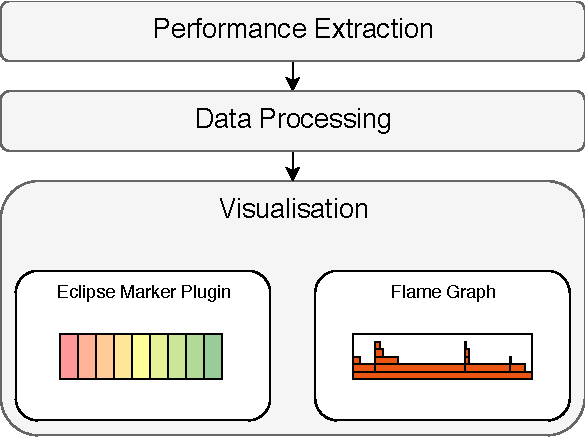
\includegraphics[width=0.7\textwidth]{images/workflow_visual_expanded}
  \caption{Visualisation Worklow.}
  \label{data_vis_workflow}
\end{figure}

The last step of our overall approach consists of novel visualisations presenting performance of configurable software systems. We wanted to support developers with tools that help identifying performance hot-spots of configurable software systems. Therefore we introduce two independent visualisation tools (overview of the tools in Figure~\ref{data_vis_workflow}), which we will present in the following.

%The last step of our approach includes visualizations of performance data (described in section~\ref{visualisation}). We designed an Eclipse plugin to visualize performance hot spots through the \ac{IDE} directly in the source code. Additionally, we used a graph-based visualisation to given an overview of the influence if configuration options on the performance of software systems.  

\subsubsection{Eclipse Marker Plugin}

The Eclipse IDE is a platform for developing in different programming languages. It is an \ac{OSS}-framework which provides mechanisms to extend it with plugins. We developed an Eclipse marker plugin which is able to highlight lines of source code inside of the eclipse workbench. The main purpose of our plugin is to highlight regions of source code to identify performance hot spots. There are different modes for highlighting implemented. First, it is able to color methods of selected configuration according to their relative performance. This might be useful if developers want to analyze default configurations of their software. The next modes color the source code according to mean and median relative performance over all configurations. These modes identify performance distribution over all sampled configurations. We are also able to color the method's configuration sensitivity. Therefore, the differences of the methods relative performance values over all configurations is calculated (we used their standard deviation). We are also able to present the workload sensitivity. This is done by calculating the standard deviation over all workloads of configurations. These different modi are selectable to a drop down menu, which is integrated in the eclipse menu-bar. To increase comprehensibility while working with this plugin we created an overview area for all modes, containing a list of all marked methods sorted by descending performance. 


%- method level visualisation
%- different modi
%- colour scheme
%- overview area
% visualisation direct in source code

\subsubsection{Flame Graphs}

\begin{figure}
  \centering
  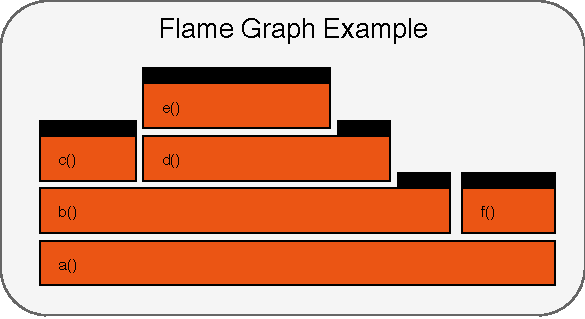
\includegraphics[width=0.7\textwidth]{images/Exampleflamegraph}
  \caption{Example Flame Graph.}
  \label{ex_flame_graph}
\end{figure}

Flame graphs are designed to visualize different non-functional properties (e.g., runtime, heap) of software systems~\cite{Gregg:2016:FG:2927299.2927301}. Flame graphs are usually presented with warm colors, because these visualisation should explain why CPUs were \textit{hot} (busy). Also the flame-like shape support this naming. Initially, they were designed to visualize the sampled stack traces\footnote{A stack trace is a list of method calls represented in a graph structure.} (which can be extracted through Linux perf\_events and DTrace). We adapted the idea of stack-trace-based flame graphs to encode the runtime of methods in flame graphs. Figure~\ref{ex_flame_graph} shows an example flame graph. The y axis encodes the call stack depth and the x axis shows the the time of methods. Each rectangle represents a stack frame (a method), where the width shows the runtime of the method in the profile. The right-to-left ordering is alphabetical. The bottom to top ordering decodes the call flow of the program. For example, function \textit{a()} from Figure~\ref{ex_flame_graph} has called the functions \textit{b()} and \textit{f()}. The top edge (black bar) of the top rectangles shows how much CPU time each has spent. That means, even if the width of \textit{b()} is bigger than the width of \textit{f()}, the latter has spent more time on CPU. With the help of these visualisations we are able to understand a whole profile in one diagram. \todo{our contribution in this field}

% control-flow graph represenation